\documentclass[a4paper,10pt]{article}
\usepackage{graphicx}
\usepackage{verbatim}
\usepackage{subfig}
\usepackage{float}
\usepackage[spanish]{babel}   %ver bien como es
\usepackage[utf8]{inputenc}
\usepackage{tabularx}
\hyphenation{des-com-po-ner-los va-rie-dad in-gre-dien-tes ac-tua-li-za-cio-nes me-dian-te con-si-de-ra-cio-nes nues-tro au-to-ma-ti-za-do pro-pues-tos con-tras-ta-das ra-zo-na-ble}

\begin{document}

\tableofcontents

\newpage


\section*{Introducci\'on}
\addcontentsline{toc}{section}{Introducci\'on}


\newpage
\section*{Presunciones}
\addcontentsline{toc}{section}{Presunciones}


\newpage


\section*{Vistas}
\addcontentsline{toc}{section}{Vistas}
En esta secci\'on presentaremos las diferentes especificaciones realizadas durante el presenta trabajo pr\'actico.
Se explicar\'a como se abord\'o cada parte del trabajo, explicando para que momentos fue utilizada cada t\'ecnica de especificaci\'on, y el porque
de esta desici\'on.

En un aspecto general, se divieron las t\'ecnicas de especificaci\'on seg\'un los siguientes crit\'erios:

\begin{itemize}
\item Modelo Conceptual: Se utilizar\'a para un entendimiento global del funcionamiento del sofware, entiendendo las entidas que interactuan dentro y con el mismo.
\item Diagrama de Casos de Uso: Se utilizar\'a para mostrar todas las interacciones que la m\'aquina tiene con los diversos actores.
\item Diagramas de Actividad: Se utilizar\'an para mostrar secuencias de acciones, usualmente agruparan diversos casos de uso que posean un hilo conductor.
\item Maquinas de Estado Finitas: Se utilizar\'an para mostrar las acciones que ocurren principalmente dentro de la m\'aquina para de esta manera, junto a los dem\'as esqumas
, poder dar un panorama completo del comportamiento del software.
\end{itemize}


\bigskip

\subsection*{Modelo Conceptual}
\addcontentsline{toc}{subsection}{Modelo Conceptual}

\subsection*{Diagrama de Casos de Uso}
\addcontentsline{toc}{subsection}{Diagrama de Casos de Uso}

Esta t\'ecnica sirve para mostrar como son las interacciones entre el mundo y la m\'aquina, es decir que se abstraen varias de las relaciones presentes
obviando las relaciones prop\'ias entre actores que se encuentran por fuera de la m\'aquina, as\'i como las interacciones que son intr\'insecas de la m\'aquina.

\subsubsection*{Diagrama}
\addcontentsline{toc}{subsubsection}{Diagrama}

A continuaci\'on se presenta el diagrama de casos de uso para toda la m\'aquina, es decir, se engloban todas las interacciones en un mismo diagrama
y luego se detallar\'a en particular cada caso de uso.


\begin{figure}[H]
\centering
\subfloat{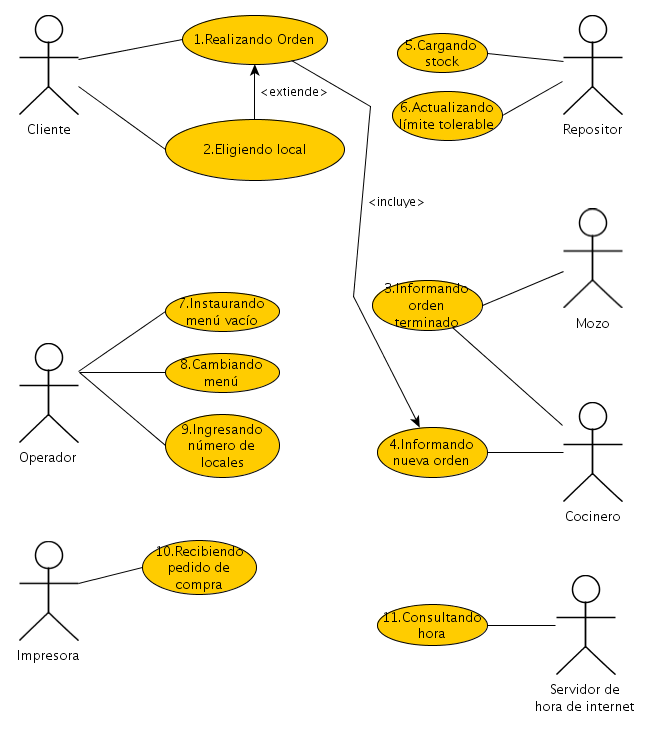
\includegraphics[width=1.3\textwidth]{Imagenes/CasosDeUso.png}}
\caption{Diagrama de Casos de Uso}
\end{figure}


\subsubsection*{Detalles Casos de Uso}
\addcontentsline{toc}{subsubsection}{Detalles de Casos de Uso}

A continuaci\'on se detallar\'a cada caso de uso, dando la descripci\'on de la sucesi\'on de hechos, adem\'as de los actores y la pre y postcondici\'on.

Para seguir un hilo conductor, los casos de uso se encuentran numerados en forma secuencial agrupados por el o los actores participantes.

Se seguir\'a este mismo secuenciamiento para realizar la descripci\'on.

Ejemplo de detalle de caso de uso
\begin{center}
\begin{tabularx}{14cm}{|X|X|}
\hline
\multicolumn{2}{|l|}{Nombre Casos de uso: Consultando archivos de ediciones pasadas}\\
\hline
\multicolumn{2}{|l|}{Actores: Periodista}\\
\hline
\multicolumn{2}{|l|}{Precondici\'on: True}\\
\hline
\multicolumn{2}{|l|}{PostCondici\'on: Se Muestra el archivo solicitado}\\
\hline
Curso Normal & Curso Alternativo\\
\hline
1.1 El periodista consulta un archivo

de edicion mediante mediante fecha

de edicion y pagina de la edicion  & 

\\
\hline
1.1.1.1 El sistema encuentra

y devuelve el articulo 

referenciado &

1.1.2.1 El sistama no encuentra 

Dicho articulo\\
\hline
1.2 Fin del CU & \\
\hline
\end{tabularx}

\end{center}

\subsection*{Diagramas de Actividad}
\addcontentsline{toc}{subsection}{Diagrmas de Actividad}

\subsection*{M\'aquinas de Estado Finita}
\addcontentsline{toc}{subsection}{M\'aquinas de Estado Finita}


\newpage


\section*{Discusi\'on}
\addcontentsline{toc}{section}{Discusi\'on}




\newpage
\section*{Conclusiones}
\addcontentsline{toc}{section}{Conclusiones}





\end{document}
